\section{Frontend}
    \subsection{UI-Design}
    Zu Beginn der Entwicklung war für BrainFlow ein Drag-and-Drop Interface angedacht, nachdem es sich herausstellte, dass es von Quasar keine Komponente gibt, die für
    ein solches Interface bestimmt ist, wurde auf eine klassische Listenansicht ausgewichen.
    
    \bigskip\noindent
    Alle Seiten von BrainFlow verwenden von Quasar zur Verfügung gestellte Components wie Buttons, Listenelemente, Suchfelder, etc.

    \subsection{Login}
        Die Login-Seite stellt ein simples Login-Eingabefeld zur Verfügung. Aufgrund von Schwierigkeiten mit der Implementierung der Nutzerauthentifizierung im Backend
        wurde die Login-Funktion nie fertiggestellt. Stattdessen leitet der Login-Button einfach auf die Notizen-Seite weiter und ein Dummy User wird initialisiert.

    \subsection{Routing}
        In Quasar müssen alle Routen in src/router/routes.js angelegt werden, diese werden als JSON-Objekt Array mit den Attributen path, component und children definiert.
        Path bezeichnet den URL-Pfad, Component die Vue Komponente, die angezeigt werden soll, und Children können weitere Routen beinhalten die einen Subpfad darstellen.
        
        \bigskip\noindent
        Quasar erstellt für SFCs die Ordner \flqq layouts\frqq, \flqq pages\frqq und \flqq components\frqq. Es gehört zu den Best Practices die höchste Komponente einer Route ein
        Layout zu machen, die Pages, die im Children-Attribut festgelegt werden, werden dann innerhalb dieses Layouts angezeigt.
        
        \bigskip\noindent
        Der Docroot unseres Development Servers; http://localhost:9000/ benutzt das LoginLayout (bis auf eine Toolbar ein leeres Layout) und weist auf die LoginPage.vue,
        während http://localhost:9000/notes/ das MainLayout benutzt (eine Toolbar mit Sidebar) und auf NotesPage.vue weist.
    
    \subsection{Notizen-Seite}
    Die Notizenseite ist die Hauptseite von BrainFlow. Sie besteht prinzipiell aus der Liste der geladenen Notizen. Die Seitenleiste wird in src/layouts/MainLayout.vue
    zusammengestellt und stellt weitere Funktionen zur Verfügung.

        \bigskip\noindent
        \begin{center}
        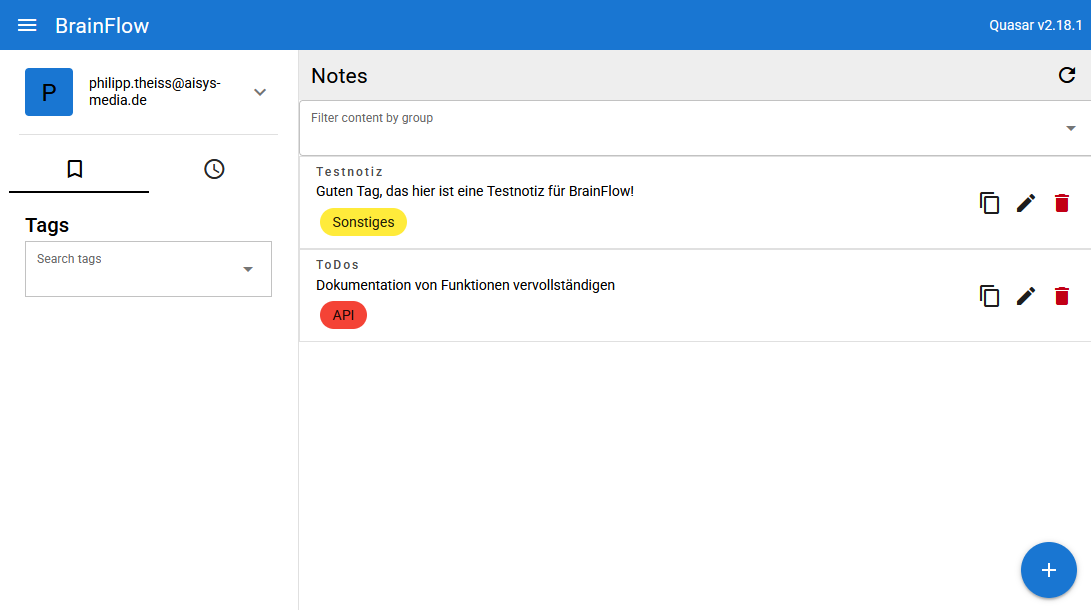
\includegraphics[width=0.75\linewidth]{ui.png}
        \end{center}
        \begin{center}
            (Abbildung \hyperref[ui]{4.1 Notizen-Seite})
        \end{center}

    \bigskip\noindent
    Vue besitzt viele nützliche Funktionen für die Arbeit mit Komponenten, z.B. kann man mit dem \flqq v-for\frqq-Parameter in einer q-list Komponente mehrere
    Listenobjekte nach derselben Vorlage erstellen. Zuvor müssen die benutzen Attribute im Script-Abschnitt definiert werden. Für Werte die sich ändern, müssen diese als
    ref() initialisiert werden, wodurch sich die Werte, die in der UI benutzt werden automatisch mit Änderung des Wertes aktualisieren.

    \bigskip\noindent
    Das Zusammensetzen von Components aus anderen Components verleiht Vue eine massive Flexibilität, die das Design und Iterieren des Frontends sehr schnell
    und frustfrei gestalten.

    \bigskip\noindent
    \begin{center}
    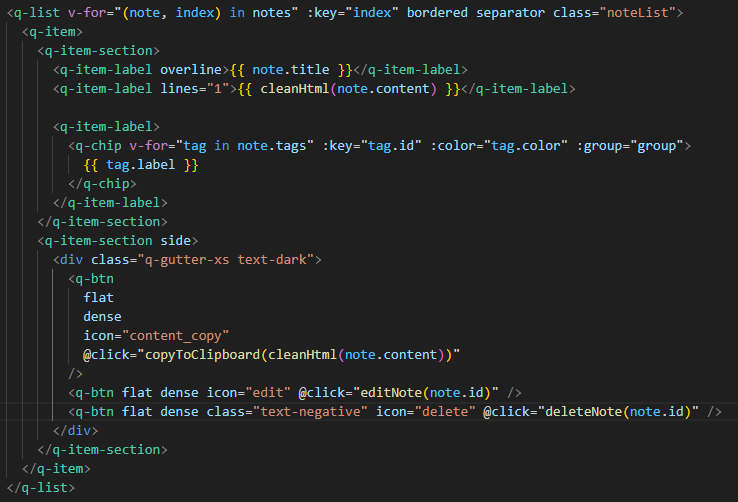
\includegraphics[width=0.75\linewidth]{notes.png}
    \end{center}
    \begin{center}
        (Abbildung \hyperref[notes]{4.2 Notizen Code})
    \end{center}

    \subsection{State Management}
        Um den Zustand der Applikation zu speichern wird der Pinia Store verwendet. In der Regel werden Pinia Stores zum ersten Mal in einer Layout-Datei
        mit einer useStore-Funktion gerufen.
        
        \bigskip\noindent
        Wenn sie erst mal initialisiert sind, bauen die useStore-Funktionen die Verbindung mit dem bestehenden Store auf und
        können deshalb ohne Bedenken von Redundanzen beliebig oft gerufen werden.

        \bigskip\noindent
        \begin{center}
            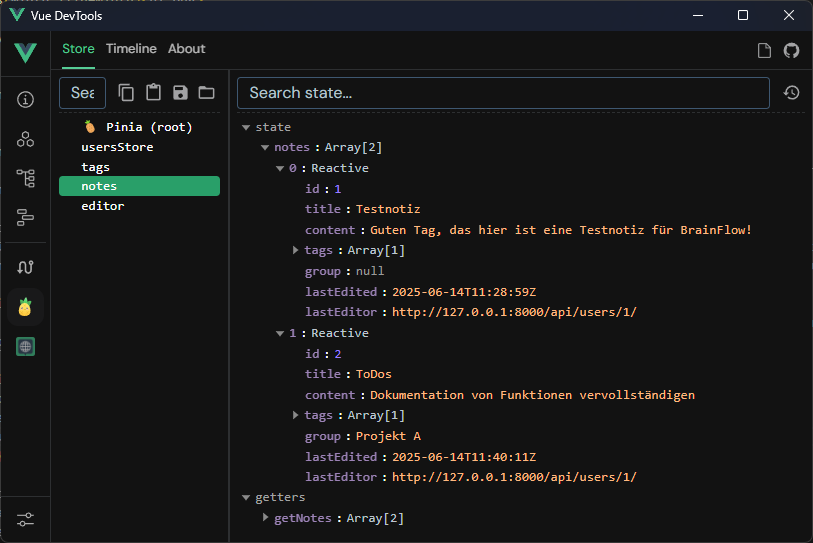
\includegraphics[width=0.75\linewidth]{pinia.png}
        \end{center}
        \begin{center}
            (Abbildung \hyperref[pinia]{4.3 Pinia State})
        \end{center}

    \subsection{CRUD-API}
        Für die API wird das Plugin Axios verwendet. In src/boot/axios.js wurde http://127.0.0.1:8000/api
        als Root URL für alle API Aufrufe festgelegt. Die Aufrufe selber sind in den Pinia Stores der jeweiligen Entitäten definiert.
        
        \bigskip\noindent
        \begin{center}
        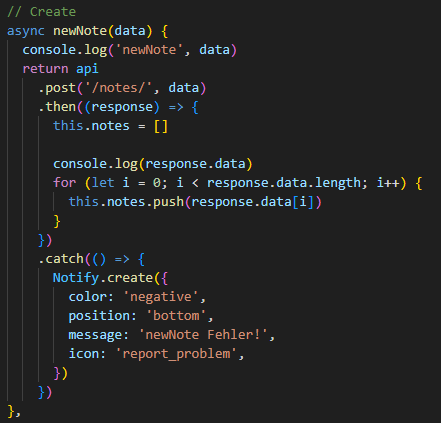
\includegraphics[width=0.5\linewidth]{api.png}
        \end{center}
        \begin{center}
            (Abbildung \hyperref[api]{4.4 Axios API})
        \end{center}

\section{Backend}
    Für das Backend wird das Python-basierte Framework Django verwendet. Obwohl Django durchaus auch Funktionen für das Routing zur Verfügung stellt, werden lediglich
    die Datenbank und API Funktionen verwendet. Das Routing im Frontend wird gänzlich von Quasar übernommen.

    \subsection{Erstellen der Datenbankmodelle}
        Die Datenbankmodelle werden mithilfe der Django ORM erstellt, wo Tabellen als Klassen definiert werden. Diese Klassen werden dann mit dem Befehl
        \flqq python manage.py makemigrations api\frqq zu SQL-Statement konvertiert, die dann mit dem Befehl \flqq python manage.py migrate\frqq ausgeführt werden.

        \bigskip\noindent
        \begin{center}
        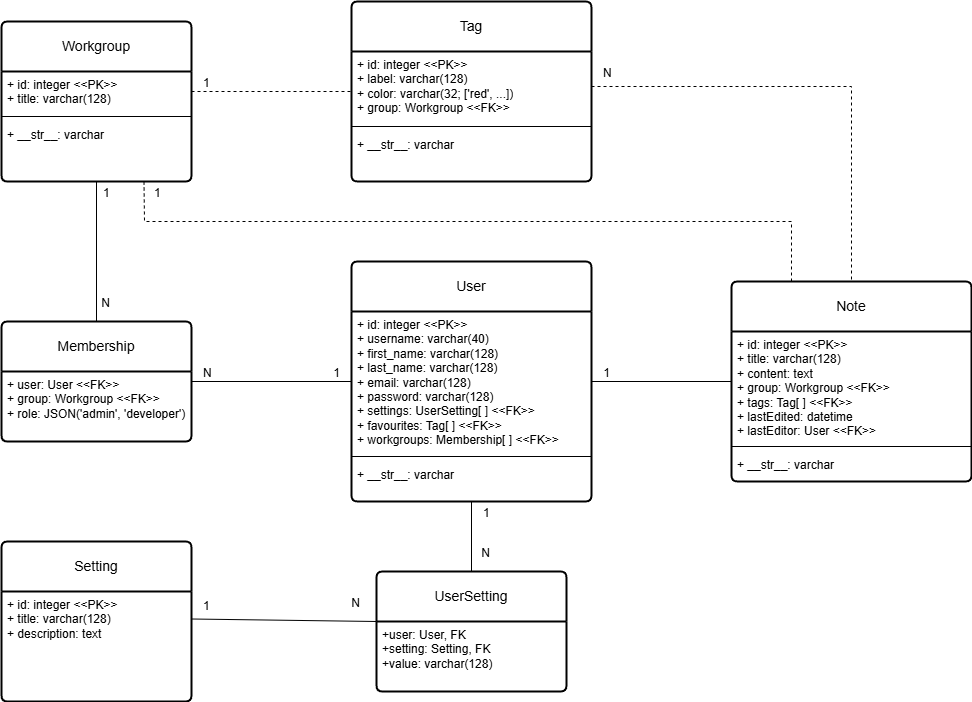
\includegraphics[width=\linewidth]{ER_Model.png}
        \end{center}
        \begin{center}
            (Abbildung \hyperref[erm]{5. ER Modell})
        \end{center}

        \bigskip\noindent
        Bei der Erstellung des Datenbankmodells wurden viele M-zu-N Beziehungen verwendet. Diese sind zwar nicht normalisiert, allerdings kann Django sie durch den
        \flqq through\frqq-Parameter Problemlos navigieren, dies wirkt sich auch auf die Einfachheit der API Implementierung aus.

        \bigskip\noindent
        Wenn eine Django-Datenbank initialisiert wird, stellt sie einige versteckte Tabellen zur Verfügung, unter Anderem eine User-Tabelle und eine Group-Tabelle. Zur Einfachheit
        der Implementierung wird die Group-Tabelle vermieden aber die User-Tabelle kann von einer selbstgemachten Klasse um weitere Datenfelder erweitert werden. Dies ist eine
        nützliche Wahl, da die Django User-Tabelle Passwortverschlüsselung mit diversen Algorithmen und User Authentifizierung unterstützt.
    
    \subsection{Administrator-Ansicht}
        Für die Verwaltung der Datenbank und das Einspielen von Testdaten wird die Django-Admin Ansicht verwendet. Hierfür muss zuvor mit dem Befehl
        \flqq python manage.py createsuperuser\frqq ein Administrator-Konto angelegt werden. Verschiedene Ansichten können dann in admin.py eingerichtet werden,
        dies muss zwar für jede Tabelle einzeln passieren aber dafür kann man steuern welche Attribute geändert werden dürfen.

        \bigskip\noindent
        \begin{center}
            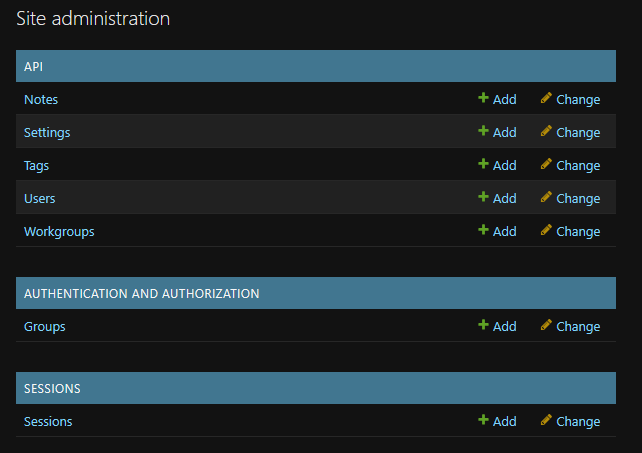
\includegraphics[width=0.75\linewidth]{admin1.png}
        \end{center}
        \begin{center}
            (Abbildung \hyperref[admin]{5.2 Admin Ansicht})
        \end{center}

    \subsection{Django REST Framework}
        Die REST-API wird mithilfe des Plugins `Django REST Framework` implementiert, dieses stellt diverse Funktionen und Klassen zur Verfügung, welche
        das Erstellen und Verwenden von Schnittstellen erheblich vereinfacht. Es kamen mehrere Klassen und Dateien zum API-Ordner dazu:
            
            \begin{itemize}
                \item urls.py: Hier wird ein Router des REST Frameworks angelegt, die bei ihm angelegten URLs werden vom Frontend angesprochen um auf das entsprechende ViewSet zuzugreifen.
                \item serializer.py: Hier werden Serializer definiert, diese wandeln die Daten aus der Datenbank in ein JSON-Objekt um.
                                    Die Klasse HyperlinkedModelSerializer orientiert sich automatisch an der Datenstruktur des gekoppelten Modells, erstellt passende CRUD-Funktionen und ist per Hyperlink ansprechbar.
                \item views.py: Hier wurden ViewSets angelegt, diese repräsentieren die Daten, die von der Datenbank geholt werden.
            \end{itemize}
        
            \bigskip\noindent
            Um M-zu-N Beziehungen aufzulösen werden außerdem bei den User, Tag, und Note Serializern SlugRelatedFields verwendet.
            Diese verweisen auf Elemente einer anderen Tabelle, allerdings unterstützt das Django REST Framework die Auflösung dieser M-zu-N Beziehungen nicht.
            Deshalb wurde das Plugin \flqq drf writable nested\frqq installiert, welches diese Beziehungen auflöst.

            \bigskip\noindent
            Der Vorteil dieser vernesteten Beziehungen, ist dass man über die Administrator-Ansicht M-zu-N Beziehungen mit Daten bestücken kann, was normalerweise nicht
            unterstützt wird. Dies hat es dem Entwickler erlaubt, einer Notiz mehrere Tags zu verleihen und die UserSettings Tabelle und Workgroup Memberships zu
            implementieren.

            \bigskip\noindent
        \begin{center}
            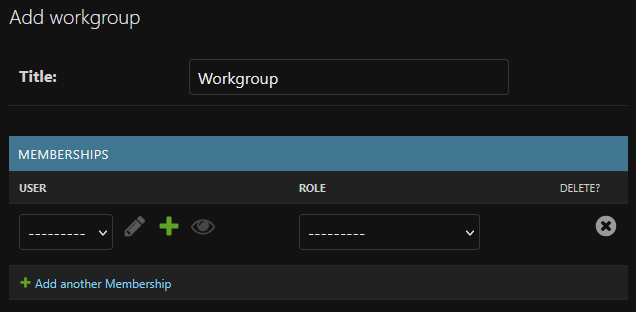
\includegraphics[width=0.75\linewidth]{admin2.png}
        \end{center}
        \begin{center}
            (Abbildung \hyperref[admin2]{5.3 Admin Menü M-zu-N })
        \end{center}